%%% mode: latex
%%% TeX-master: t
%%% End:
\chapter{绪论}
\label{cha:intro}

本章围绕海上雾天无人机小目标检测问题，系统阐述研究背景与现实需求，分析该技术的应用价值。随后，概述通用目标检测、针对海上无人机图像的小目标检测、图像去雾技术以及复杂雾天场景下的目标检测方法的国内外研究进展，并深入分析当前存在的问题与挑战。最后给出本文的研究内容与章节安排。

\section{研究背景与意义}
海洋强国战略是我国重要发展方向。开放水域覆盖了地球 70\% 以上的面积，承载着全球约 80\% 的国际贸易\cite{ref1}。近年来，面向海洋环境的无人机与无人水面艇平台部署规模持续增长，海洋科学家使用各种传感器收集大量视觉数据，因此迫切需要稳健可靠的方法来进行量化、检测、分类和理解。近几十年来，人们在开发水面和水面以上运行的自主机器人方面投入了大量精力，计算机视觉在海洋和淡水领域的应用发展迅速。为在交通繁忙或靠近海岸的水域实现精确导航，计算机视觉愈发重要。在此背景下，学术界逐渐形成面向海洋视觉感知问题的研究方向。例如，MaCVi\cite{ref2} 研讨会旨在推动现代计算机视觉方法在多种空中和水面领域的应用，例如海上搜索和救援、海上巡逻、船舶石油和污水泄漏监测、垃圾检测等。
所有这些应用均依赖于高性能的无人机与无人水面艇视觉系统。视觉系统效能的发挥直接依赖于对无人机航拍图像进行高效且准确的目标检测。尽管近年来基于深度学习的目标检测技术在智能交通、自动驾驶等陆地自然场景中取得了突破性进展，但大多数先前模型是为自然场景图像设计的，对于中大型物体有良好的检测结果。然而直接将现有的常规视觉模型应用于环境复杂的海上无人机航拍场景，往往出现检测精度下降与误检漏检增多等问题。

这种局限性主要源于复杂的现实因素。首先，复杂气象条件对光学成像造成了严重干扰。受洋流与大气环流影响，海洋气候复杂多变，海面易产生平流雾、辐射雾等气象现象。根据经典大气散射成像模型，可见光在传播过程中受到悬浮颗粒的散射与吸收作用，成像结果可视为场景辐射衰减项与空气光叠加项的组合，导致航拍图像产生明显的对比度衰减与细节损失现象。这种退化首先表现为图像对比度的显著下降，使得目标与海面或天空背景的边界信息显著弱化。其次，光学散射会导致严重的颜色失真与饱和度降低，致使图像丢失丰富的色彩辨识信息。更严重的是，浓雾会遮蔽目标的高频细节纹理，使得距离无人机较远的微小目标难以与灰白色的背景噪声区分。雾气的存在削弱了现代深度学习检测算法赖以识别目标的底层语义特征，导致常规模型在雾天环境下易发生大量漏检。

除复杂气象条件影响外，海上无人机航拍目标检测任务本质上属于小目标检测问题。而小目标检测主要针对尺寸较小、在图像中占比很小的目标实例进行精准分类和定位。相比于大目标检测,小目标检测在实际应用中面临着更大的挑战。由于小目标本身尺寸较小，经过基础网络下采样后，目标信息会被大幅度压缩甚至丢失。同时，小目标由于在图像中占据的面积很小，即使是微小的像素级别偏移，也会显著影响检测准确性。

不可预测的海洋动态背景与严苛的端侧硬件限制进一步加剧了检测任务的难度。即便在能见度良好的无雾环境，海面本身也是一个高度动态且充满干扰的复杂背景。无规则起伏的波浪、翻滚的白色海洋泡沫，以及在标准光学相机和多光谱相机中极易产生的强烈太阳反射高光伪影，会导致输入图像的局部信噪比较低。海事搜救与巡逻任务对算法的实时性提出严格要求。

综上所述，在复杂天气下提高海上无人机鲁棒的视觉感知能力，让其能够独立准确地完成小目标检测任务，在理论建模与工程实现层面均具有较高研究难度。研究一种既能有效对抗雾气干扰又兼顾小目标检测精度与端侧实时性的算法，具有重要的学术研究价值和实际工程意义。


\section{国内外研究现状}
\label{sec:related_work}
本节将从通用目标检测算法、面向海上无人机图像的小目标检测方法、图像去雾技术，以及复杂雾天场景下的目标检测方法四个维度，详细梳理国内外相关领域的研究进展，并分析现有方法存在的局限性。

\subsection{通用目标检测算法研究现状}
近些年来随着深度学习技术的不断进步,目标检测正在应用于各个领域,包括车辆检测、人脸检测、船舶检测等。大多数基于深度学习的目标检测方法都基于卷积神经网络架构,这些架构被用于从输入图像中提取特征。以深度学习为基础的目标检测算法分为 Two-stage 目标检测算法,One-stage 目标检测算法以及基于 Transformer 的目标检测算法,近年来出现的经典模型如图1-1所示。Two-stage 目标检测算法先通过区域建议产生感兴趣区域,然后进行候选区域的特征提取、分类回归等操作。One-stage 目标检测算法是一种基于回归的检测算法,因此不需要历经候选区域的生成这一步骤。基于Transformer 的目标检测算法与传统的卷积神经网络检测器不同,直接使用自注意力层处理特征信息,摆脱了对手动设计的锚框和区域提议网络的依赖。
\begin{figure}[!htbp]
    \centering
    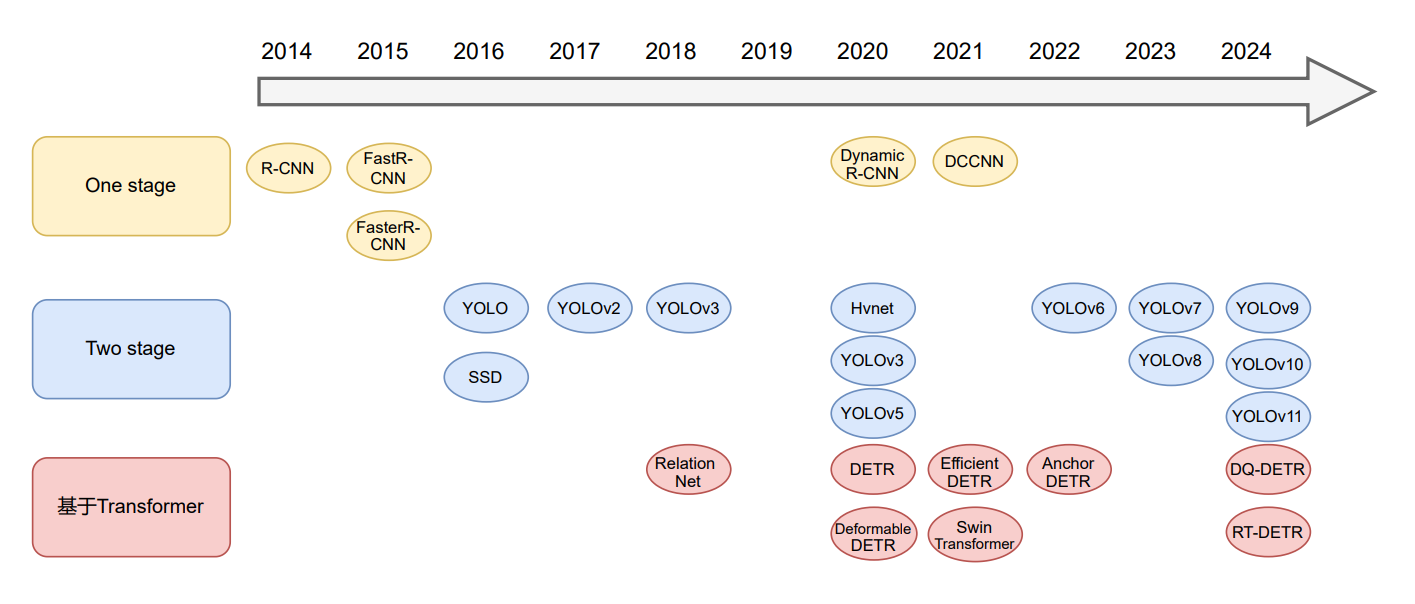
\includegraphics[width=0.9\linewidth]{figures/近年来的经典通用目标检测算法模型.png}
    \caption{近年来的经典通用目标检测算法模型}\label{Fig1-1}
\end{figure}

在早期的深度学习目标检测研究中，双阶段目标检测算法占据主导地位。其核心思想是将复杂的检测过程拆解为区域建议提取和特征分类及边界框回归两个独立的步骤。基于区域的卷积神经网络 R-CNN\cite{ref3} 是该领域的经典方法，它采用新的选择性搜索方法在输入图像中生成大量候选区域，并首次利用卷积神经网络对这些区域逐一提取特征。针对早期算法计算高度冗余的缺点，He 等人\cite{ref4} 提出了空间金字塔池化网络算法，通过在整张特征图上进行池化操作缓解了输入尺寸的限制。随后 Fast R-CNN\cite{ref5} 利用原图与特征图的映射关系实现了特征共享与多任务联合训练。在此基础上，Faster R-CNN\cite{ref6} 引入了区域生成网络取代选择性搜索，将目标检测的所有环节统一在单一网络中，实现了端到端训练模式。在此基础之上，研究者针对特定领域进行了大量改良。例如 Chen 等人\cite{ref7}使用双通道卷积神经网络加入虚警可控分类器，以期提高海面雷达目标的检测性能。Zhang 等人\cite{ref8} 提出了 Dynamic R-CNN 以动态调整训练过程中的标签分配标准。尽管双阶段算法在特征对齐与定位精度上表现优异，但其串行的网络拓扑结构导致检测速度较慢，且模型参数量普遍较大，难以满足无人机等边缘计算设备对低延迟和高帧率的严格要求。

为了克服双阶段算法的速度瓶颈，单阶段检测算法应运而生。Redmon 等人\cite{ref9}提出了单阶段代表性模型 YOLO，该模型舍弃了区域建议步骤，将目标类别概率和边界框坐标的预测转化为纯粹的回归问题。随后该系列算法进入了快速发展阶段。YOLOv2\cite{ref10} 和 YOLOv3\cite{ref11} 引入了多尺度训练策略、批量归一化机制以及特征金字塔网络，提升了模型对不同尺度物体的感知能力。YOLOv4\cite{ref12}和 YOLOv5\cite{ref13} 在数据增强技术、损失函数设计和工程轻量化部署方面做出了贡献。新一代算法如 YOLOv6\cite{ref14} 到 YOLOv10\cite{ref18} 不断在网络架构设计和参数量压缩上进行优化。最新的 YOLOv11 通过引入具有空间注意力的跨阶段局部模块，提升了复杂场景下遮挡物体的检测能力。除了 YOLO 家族，SSD\cite{ref19} 和 HVNet\cite{ref20} 等经典算法也在兼顾推理速度与多尺度特征融合方面取得了成效。然而，单阶段算法追求速度的本质决定了其在网络加深或进行下采样时易出现高频细节丢失的现象。这种特征流失对特征本就微弱的小目标检测而言会面临精度瓶颈。


传统的卷积神经网络受限于局部的卷积核感受野，难以充分对图像中远距离目标间的全局依赖关系进行有效建模。随着自注意力机制的引入，目标检测领域迎来了新的发
展。RelationNet\cite{ref21} 率先尝试利用注意力机制对不同目标间的关系进行建模。随后 DETR 算法\cite{ref22} 被提出，它将目标检测转化为集合预测问题，
利用二分图匹配的匈牙利算法促使网络输出唯一的预测框，有效避免了锚框设计和非极大值抑制等依赖人工经验的后处理组件。为了提升变换器在小目标检测上的表现并
加速模型收敛，Deformable DETR\cite{ref23} 引入了可变形卷积以关注关键特征区域。Efficient DETR\cite{ref24} 和 Anchor-DETR\cite{ref25} 通过不同的先验设计减少了背景噪声的干扰。DQ-DETR\cite{ref26} 和基于滑动窗口的 Swin Transformer\cite{ref27} 增强了模型在多尺度下的细粒度特征提取能力。近期由百
度团队提出的实时端到端检测器 RT-DETR\cite{ref28} 通过设计高效的混合编码器结构，克服了传统自注意力架构计算复杂度随序列长度呈平方级增长的问题。该模型
在资源受限的情况下实现了实时高帧率检测，在小目标召回率上展现出了优越性能，成为复杂背景下目标检测的理想基准架构。

\subsection{面向海上无人机图像的小目标检测方法研究进展}

前文所述的通用目标检测算法大多针对视野平行且目标清晰的陆地自然场景设计，在直接面对海上无人机航拍图像时往往存在严重的适应性不足。海事无人机视角的特殊性集中体现在目标像素极小、同类目标尺度变化剧烈、海浪高光干扰严重以及机载平台算力极度受限。为此学术界针对这些特殊性展开了大量具有针对性的深度研究与架构改良。

针对海上目标尺度跨度极大多样性的挑战，尺度感知特征融合方法被广泛应用。从早期的图像金字塔\cite{ref29, ref30}方法发展到特征金字塔网络\cite{ref31}，通过建立自上而下的跳跃连接融合深层高维语义与浅层高频细节，成为了处理尺度变化问题的基石方案。在此设计思想的基础上，FSSD\cite{ref32}算法重构了底层特征以生成一系列更加丰富的特征金字塔。Liang等人\cite{ref33}和Liu等人\cite{ref34}通过精巧设计的反卷积层成功剥离了多尺度融合过程中的冗余信息。专门针对无人机航拍图像的特性，Trident-FPN\cite{ref35}结合了不同感受野的特征图以适应目标尺度。NETNet\cite{ref36}则开发了一种邻居特征擦除机制，用以避免大目标的深层强语义在融合时对微小目标微弱特征造成的负面干扰或淹没。尽管这些尺度感知方法在一定程度上缓解了漏检问题，但极其复杂的跨层特征融合通常会显著增加内存占用与计算负担。

\begin{figure}[!htbp]
    \centering
    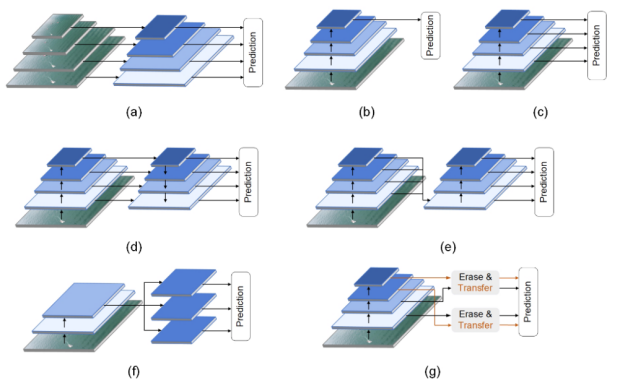
\includegraphics[width=0.9\linewidth]{figures/尺度特征提取方法对比.png}
    \caption{尺度特征提取方法对比}\label{Fig1-2}
\end{figure}


为了缓解深层卷积池化操作导致的小目标特征消失问题，研究者们提出了特定的小目标检测优化与注意力补偿机制。Mandal等人\cite{ref37}设计了轻量级的AVDNet，通过引入多尺度残差块结构来确保小目标显著特征在深层网络中的高质量表征传递。Yang等人\cite{ref38}则提出了QueryDet框架，巧妙地采用级联稀疏查询机制，首先在低分辨率的深层特征上预测目标的粗略位置，随后依靠该位置信息引导网络在高分辨率浅层特征上进行局部精确计算，有效避免了对大面积无效海洋背景的冗余计算。尽管此类局部上下文建模方法有效提升了微小目标的召回率，但其引入的额外查询与匹配操作依然增加了网络的运行开销。

鉴于海事无人机和无人水面艇的有效载荷与电池容量极为有限，面向移动边缘端侧的轻量级网络架构设计成为必然趋势。MobileNet\cite{ref39}和ShuffleNet\cite{ref40}等极具代表性的轻量级骨干网络通过深度可分离卷积运算和跨通道洗牌等技术极大减少了模型的前向推理参数量。基于这些高效的骨干网络，研究者开发了诸如YOLO-Lite\cite{ref41}和ShuffleDet\cite{ref42}等专门针对无人机航拍的实时检测模型。Zhou等人\cite{ref43}提出的SE-YOLOv3引入了空间注意力模型压缩冗余背景信息以突出目标响应。Zhao等人\cite{ref44}针对海面微小物体改进的模型在特定的公开海事数据集上显著提升了检测精度。然而上述所有轻量化优化方法几乎都隐含了一个严苛的假设，即输入图像处于理想的清晰视觉状态。一旦真实的海洋环境出现大雾等复杂天气，这些轻量级网络本来就极其有限的特征拟合能力往往会面临衰减甚至失效的问题。

\subsection{图像去雾技术研究进展}

在复杂多变的实际海上应用环境中，雾气是导致图像视觉特征严重退化的重要环境因素。对受雾气干扰的图像进行去雾处理是提升下游目标检测、多目标跟踪等高级视觉任务精度的关键预处理与特征重构环节。纵观发展历程，目前的去雾技术大致经历了传统图像增强、物理先验理论建模以及深度学习数据驱动方法三个主要阶段。
\begin{figure}[!htbp]
    \centering
    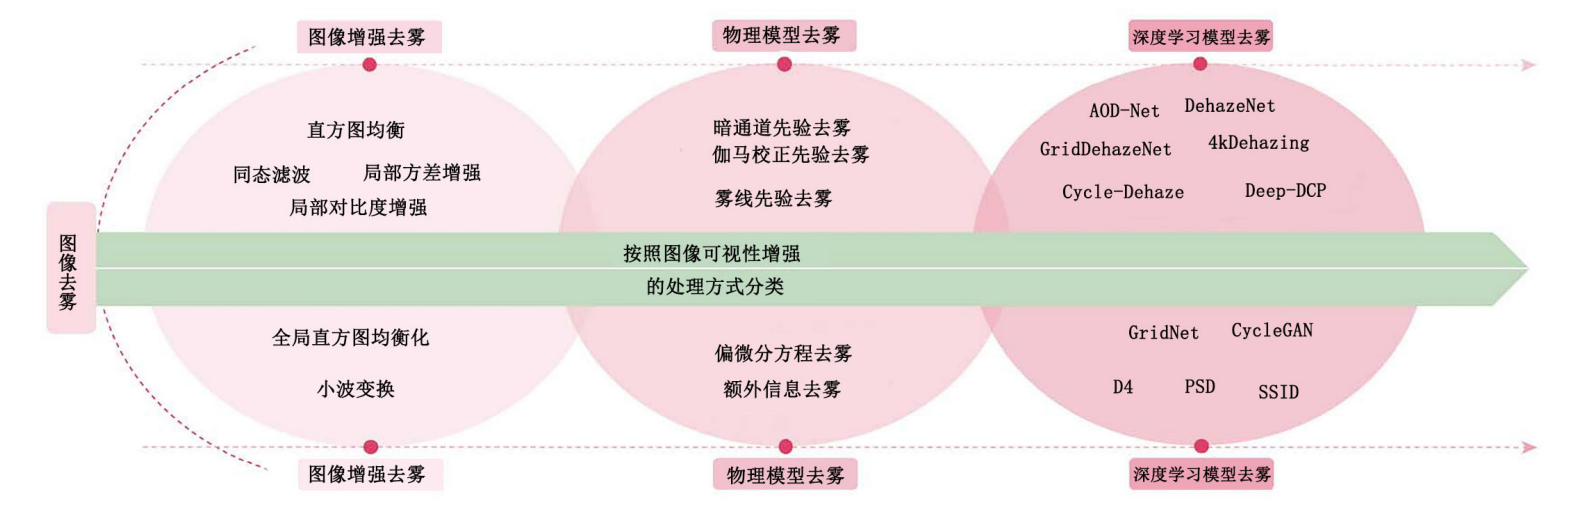
\includegraphics[width=0.9\linewidth]{figures/图像去雾技术发展.png}
    \caption{近年来的经典图像去雾算法及模型}\label{Fig1-3}
\end{figure}
早期的图像去雾主要依赖于传统的图像增强算法，这类算法往往忽略了雾气产生的光学物理本质，而是直接从图像处理的角度对像素的亮度、全局对比度和色彩饱和度进行强制调整。其中最典型的直方图均衡化技术通过横向拉伸灰度分布来放大图像的细节轮廓，但Karel等人\cite{ref50}在研究中指出其极容易导致非雾区域的强度过曝和整体颜色严重失真。随后学术界相继提出了各种改进的自适应直方图均衡化方法\cite{ref51, ref52}，试图通过子块重叠和对比度限制来抑制过度增强。同态滤波技术\cite{ref53}尝试在频域空间内分离并调整图像的光照分量以改善对比度。多尺度色彩恢复理论\cite{ref54, ref55, ref56}则试图通过模拟人类视觉系统的感受机制分离环境光与物体反射属性。然而此类方法普遍缺乏物理依据，往往会在图像边缘及深度突变处产生极不自然的光晕效应和强烈的色彩失真，从而对下游视觉任务的语义建模产生不利影响。

随着对大气悬浮颗粒物理光学散射成因研究的不断深入，基于严谨大气散射模型的方法逐渐成为代表性工作。Narasimhan等人\cite{ref58}通过采集多幅同场景图像成功推导出了场景的光学深度。Fattal\cite{ref60}则独辟蹊径地通过独立成分分析算法尝试消除图像中的环境散射光。这一发展阶段中具有代表性的成果之一是He等人\cite{ref61}提出的暗通道先验理论。该方法通过统计规律惊奇地发现户外无雾图像在非天空区域至少存在一个极低灰度值的颜色通道，据此成功估算出高精度的透射率分布图并反演出清晰的去雾图像。随后曾接贤等人\cite{ref62}进一步结合双边滤波技术显著提升了该算法的保边平滑性能。但物理统计先验并非万能，在面对海上强烈的阳光水面反光或占据画幅大半的明亮天空等完全不满足暗通道统计假设的特殊区域时，该算法往往会面临严重的参数估计失效，导致去雾后的复原图像出现大面积的颜色发黑与视觉假影。

近年来，随着硬件算力的突破和大规模成对数据集的涌现，基于深度学习的数据驱动去雾算法成为了学术界和工业界绝对的主流方向。Cai等人\cite{ref63}提出的DehazeNet首次使用深度卷积神经网络直接从单幅有雾图像中非线性地映射出透射率图。Ren等人\cite{ref64}紧随其后采用了多尺度卷积网络架构进行透射率的粗细化递进估计。Li等人\cite{ref65}的研究则在结构设计方面进行改进，将透射率与大气光强统一整合为一个综合参数，从而实现了一个完全端到端直接输出清晰图像的重构网络，并开源了著名的综合去雾基准数据集\cite{ref66}。随着生成对抗网络理论的成熟与完善，多项前沿研究\cite{ref69, ref71}通过循环一致性损失成功实现了无需成对样本监督的真实雾天去雾。同时，具备强大全局感受野的先进序列建模架构\cite{ref72}也被尝试引入去雾领域以获取全图的上下文依赖，但其自注意力机制极高的计算复杂度使其无法直接处理无人机高分辨率航拍图像。最新兴起的状态空间模型凭借其选择性扫描机制，在保持全局感受野的同时将时间复杂度降至线性级别，这为在无下采样的前提下提取高分辨率物理去雾提供了新的研究思路。

\subsection{复杂雾天场景下的目标检测}
对有雾环境下的目标检测任务，常规的通用视觉检测模型在清晰场景下表现良好，但在复杂雾天环境下往往存在显著的性能衰减问题。近年来，随着单阶段检测器与端到端集合预测框架的快速发展，诸如YOLOv7、YOLOv8、YOLOv12以及RT-DETR等基线模型在特征提取效率与检测精度上取得了较好的平衡。然而，这类纯数据驱动的通用模型主要依赖于清晰目标的局部纹理与几何边缘，在应对海面非均匀雾气遮挡时，缺乏显式的抗退化机制，容易出现微小目标特征弱化与背景语义混淆，导致召回率下降。为了解决这一问题，目前前沿的研究倾向于采用去雾预处理、域适应或多任务联合学习等框架，以提升模型在恶劣天气下的感知鲁棒性。

前置去雾预处理策略是早期提升雾天目标检测性能的常见方法。该类策略通常通过独立的去雾模型对图像进行增强后再送入检测器，例如采用基于物理先验或深度学习图像复原级联的C2PNet与RIDCP等预处理方案。这类方法能够一定程度地恢复图像的整体对比度与视觉清晰度。然而，低级图像去雾模型的优化目标通常侧重于人类视觉感官层面的峰值信噪比或结构相似度，并未针对下游的检测任务进行特定的特征约束。在处理微小目标时，这种像素级的平滑去雾操作往往会造成目标高频边缘与几何纹理的不可逆丢失。此外，两阶段独立级联框架引入了额外的图像重建计算开销，难以满足无人机等机载平台的低延迟实时处理需求。

为了克服独立级联框架的局限性，部分研究转向域适应与多任务联合学习策略。域适应方法试图在特征层面对齐清晰域与雾天域的分布，例如采用在线去雾与特征级域适应策略的MS-DAYOLO，以及基于网络结构优化与多模态特征融合的DA-Detect与YOLOv5s-Fog等模型。此外，一些研究利用改进的架构探索了恶劣天气下的目标检测问题，如D-YOLO利用双分支网络与特征自适应融合来增强雾霾条件下的鲁棒性，FogGuard利用感知损失与合成数据增强提高了检测准确率。尽管这些方法在一定程度上提升了复杂环境下的检测性能，但现有的联合框架多采用隐式的特征对齐或图像级参数耦合策略，往往未能将去雾网络中间层提取的丰富物理环境特征直接注入到检测网络的深层语义提取层中。由于缺乏显式的物理去雾特征监督，这种特征信息流的截断限制了模型对浓雾遮挡目标的召回能力，且在面对特定小样本数据集时容易引发过拟合现象。

针对雾天物理退化特征的提取，基于频域解耦与状态空间建模的方法近年来展现出一定的潜力。雾气在图像中的分布通常表现为低频的平缓变化，而目标结构则集中于高频细节。状态空间模型在长序列建模与全局信息聚合方面表现出较强的能力。例如，WDMamba通过结合小波分解与状态空间建模，在图像复原任务中有效增强了多尺度信息交互与退化先验的提取能力。Fourier-RWKV等网络则从频域建模角度探讨了全局信息表达的提升。这类方法在处理非均匀物理退化时具有明显的架构优势，但目前尚未充分应用于海上无人机雾天小目标检测的特征级融合场景中，如何利用其线性复杂度的优势来指导检测器进行定向特征补偿仍有待进一步探索。

综上分析，现有方法在应对算力受限的海上雾天小目标检测场景时仍面临诸多挑战。单阶段模型推理速度快但对雾天微小目标易漏检，基于复原的大型模型检测精度尚可但算力开销过大，轻量化网络抗背景干扰能力较弱，而传统的域适应与两阶段模型在物理特征利用与泛化能力上存在局限。与部分侧重于城市自动驾驶或通用户外感知的现有研究不同，本文的工作聚焦于海上无人机航拍的独特需求。如何在已有的通用目标检测模型基础上，通过显式的物理先验提取与轻量化架构重构，实现有雾环境下目标检测精度、跨域泛化能力与端侧推理延迟之间的有效平衡，仍是一个需要不断探讨的课题。本文旨在通过多维注意力机制与频域状态空间模型的协同设计，为这一问题提供可行的优化方案。


\section{论文研究内容}
\label{sec:research_content}

针对现有工作的不足，以及前文提到的海上雾天环境下无人机航拍小目标检测面临的数据匮乏、目标尺度小、雾气退化严重以及端侧算力受限等痛点问题，本文围绕数据集构建、轻量化特征提取优化以及物理引导的特征级去雾融合三个核心维度开展研究工作。本文的主要研究内容如下：

{（1）雾天海上小目标数据构建方法研究}。针对真实雾天成对监督数据在物理空间中难以获取的工程难题，本文在公开的海上航拍数据集基础上，引入单目深度估计模型提取场景的相对深度信息。基于经典的大气散射模型，本文构建了严密的雾天物理成像退化过程。通过平滑调节雾气浓度参数与全局大气光强度，并结合高斯模糊策略，批量生成了包含轻雾、中雾和浓雾等多种能见度级别的高质量合成数据集。所构建的多源异构数据集为本文算法在雾天环境下的感知鲁棒性验证、模型多阶段联合训练以及最终的客观性能评估提供了坚实的数据基础。

{（2）面向小目标的轻量化目标检测网络优化}。针对无人机机载算力严重受限与小目标特征易在深层网络中流失的矛盾，本文以实时端到端检测框架 RT-DETR 作为基准模型进行轻量化重构。在语义特征提取阶段，采用轻量级残差网络作为主干以大幅降低计算复杂度；同时在残差模块内部创新性地嵌入无参数三维能量注意力机制与倒残差多头自注意力模块，从底层特征维度有效抑制海面反光等动态背景噪声，并显著放大了微小目标的高频响应。此外，在特征融合编码器中引入级联分组注意力机制，改善了多尺度特征的空间交互效率，从根本上提升了小目标的定位精度与端到端检测的收敛稳定性。

{（3）雾分布表征与特征增强分支设计与物理引导融合方法研究}。针对非均匀雾气退化对深层语义特征表达的破坏性影响，本文设计了基于频域解耦与状态空间模型的雾分布表征增强分支。该分支利用二维离散小波变换剥离低频物理退化成分，并依托状态空间模型的线性全局建模能力，稳定提取反映空间雾气浓度的特征图。在此物理先验的基础上，本文构建了动态物理引导特征融合模块，通过空间残差与通道注意力双重机制，利用低频环境先验精准引导高频几何细节的特征补偿。为保障多任务优化的稳定性，本文配套提出了分阶段协同训练策略，通过先验分支独立预热与检测器解耦微调，建立了物理退化先验与视觉语义识别的协同工作链路。

\section{论文组织结构}
依据实际开展研究工作的过程，本文将分为五个章节进行内容组织：

第一章，绪论。本章首先强调在海上有雾环境下提高无人机小目标精准检测能力的迫切需求。接下来通过广泛阅读国内外文献资料，分类梳理出四大相关领域的技术发展与国内外研究现状，并整理相关技术存在的问题和不足，引出本文的研究方向。最后总结本文主要研究内容和各章节安排。 

第二章，海上雾天无人机图像退化机理分析与数据集构建。本章从大气散射成像模型出发，分析雾天图像的形成机制及其对小目标视觉特征表达能力的影响；进一步从频率角度探讨雾天图像高低频分布特性，引入小波分解理论，为后续雾分布表征与特征增强分支设计提供理论支撑。在此基础上，提出基于物理先验的海面非均匀雾模拟方法，并构建面向海上小目标检测任务的雾天数据集，为模型训练与实验评估提供可靠数据基础。

第三章,面向海上雾天场景的轻量级目标检测模型设计。本章在所选端到端目标检测框架基础上，针对雾天小目标易退化、特征表达不足等问题进行结构优化。首先通过改进轻量化主干网络并引入多维注意力机制提升微小目标特征表达能力；其次构建基于状态空间模型的雾分布表征与特征增强分支，以实现雾天细节信息的有效恢复；随后设计动态物理引导特征融合机制，加强环境先验与语义信息的协同表达；最后提出分阶段协同训练策略，以保障联合模型的稳定收敛与性能提升。

第四章,实验与结果分析。本章首先介绍海上雾天目标检测数据集的构建细节、实验评价指标及实验环境配置。随后通过基线对比实验、主流算法对比实验以及关键模块消融实验，系统评估本文模型在不同数据集下的检测性能。最后结合定量指标与可视化结果，对模型在复杂海上雾天环境中的鲁棒性与泛化能力进行分析。

第五章为总结与展望。本章对本文围绕海上雾天小目标检测问题所开展的研究工作进行系统总结，客观分析模型在实际应用中的局限性，并展望未来在非均匀团雾自适应检测策略及模型高效部署等方面的进一步研究方向。








